\documentclass[a4paper, 14pt]{extarticle}


% ====== Localization & fonts ======
\usepackage{xcolor}
\usepackage{fontspec}
\usepackage{polyglossia} % Russian lang
\setdefaultlanguage{russian}
\setmainfont{Times New Roman}
\newfontfamily\cyrillicfont{Times New Roman}

% TODO look for better; don't like this one
\setmonofont[Scale=0.9]{DejaVu Sans Mono}
\newfontfamily{\cyrillicfonttt}{DejaVu Sans Mono}[Scale=0.8]

% ====== Page layout ======
\usepackage[ % Margins
left=1cm,
right=1cm,
top=2cm,
bottom=2cm	
]{geometry}

% ====== Document sectioning ======

\usepackage{titlesec}

\newcommand\sectionbreak{\clearpage} % Each section on a new page

\titlespacing*{\paragraph}{0pt}{15pt}{6pt}
\titlespacing*{\subparagraph}{0pt}{15pt}{3pt}

% ====== Math ======
\usepackage{amsmath} % Math stuff
\usepackage{gensymb}

% ====== Other text spacing ======

\usepackage{setspace} % String spacing
\onehalfspacing

\usepackage{parskip} % The red line
\setlength{\parskip}{15pt} % Sep beetween paragraphs

\usepackage{enumitem}
\setlist{nosep, topsep=-10pt} % Remove sep-s beetween list elements

% ====== Source code listings ======

\usepackage{listings} % Source code
\lstset{
	basicstyle=\ttfamily,
	breaklines=true,
	breakatwhitespace=true,
	commentstyle=\color{green},
	keywordstyle=\bfseries\color{blue},
	tabsize=4
}

\lstdefinestyle{num}{
	numbers=left,
	numbersep=0.5cm,
	numberstyle=\ttfamily,
	xleftmargin=0.85cm,
}

\lstdefinestyle{framed_num}{
	frame=single,
	numbers=left,
	numbersep=0.5cm,
	numberstyle=\ttfamily\color{red},
	xleftmargin=1cm,
	framexleftmargin=1cm
}

\lstdefinestyle{sql_style}{
	morekeywords=[10]{while, do, procedure, begin, end, if, tinyint, enum, datetime, boolean}
}

% ====== CSV ======
\usepackage{csvsimple} % Load CSV

% ====== References ======
\usepackage{hyperref} % Links
\hypersetup{
	colorlinks,
	citecolor=black,
	filecolor=black,
	linkcolor=black,
	urlcolor=black
}

% ====== Headers ======
\usepackage{fancyhdr}
\pagestyle{fancy}
\fancyhead[L]{}

% ====== Misc ======
\usepackage{metalogo} % Logos for LaTeX
\usepackage{lipsum} % Lorem ipsum
\usepackage{graphicx} % Pictures
\usepackage{tabularx} % X-tables
\usepackage{csquotes} % French quoutes
\usepackage{caption}
\usepackage{subcaption}
\usepackage{lastpage}

\usepackage{placeins} % FloatBarrier
\captionsetup[figure]{name=Рисунок, labelsep=endash, parskip=0pt}

% ====== My commands ======
\newcommand{\addonsubheader}[1]{{\center{\bfseries \vspace{-0.5cm} #1} \\ \vspace{15pt}}}

\newcommand{\definition}[1]{\textbf{#1}}
\newcommand{\screenshot}[3]{
	\begin{figure}[h]
		\centering
		\includegraphics[#1]{#2}
		\caption{#3}
	\end{figure}
}

% ====== Counters ======

\newcounter{stepcounter}[subsubsection]

\newcommand\steppar[1][\DefaultOpt]{
	\def\DefaultOpt{#1}
	\paragraph{Шаг №\thestepcounter.}
	\refstepcounter{stepcounter}
}

\begin{document}
	\begin{titlepage}
		{\centering
			{\bfseries
				
\includegraphics[height=8cm]{logo.jpeg}\\
				Unity. Precision. Perfection.\\
				\vspace{3.5cm}
				\uppercase{Конспект лекций} \\
				по дисциплине \enquote{Компьютерная графика}\\
			}
			\vspace{\fill}
		}
		\begin{tabular}{l l}
			\textbf{Лектор}: & Герасимова Тамара Владимировна\\
			\textbf{Страниц}: & \pageref{LastPage}\\
			\textbf{Последнее обновление}: & \today{}\\ 
			\textbf{Автор}: & Корытов Павел, 6304\\
		\end{tabular}
	
		\vspace{2cm}
		{\centering
			Санкт-Петербург \\
			\the\year\\
		}
	\end{titlepage}

\tableofcontents
\newpage
\section{2D преобразования}
\subsection{Геометрические преобразования в	компьютерной графике}
Преобразования в КГ:
\begin{itemize}
	\item Проекционные
	\item Геометрические
	\begin{itemize}
		\item Афинные
	\end{itemize}
\end{itemize}
В машинной графике представлена большая группа геометрических преобразований (аффинная группа): перенос, поворот, масштабирование. Геометрические преобразования позволяют изменять и визуализировать объект.

Компьютерная графика имеет дело со множеством геометрических объектов, таких как точки, многоугольники и многогранники. Все разнообразие геометрических объектов можно свести к ограниченному множеству простейших сущностей. Нам понадобятся для этого три базовых типа — скаляры, точки и векторы.

Существуют, по крайней мере, три варианта определения этих сущностей, в зависимости от того, с какой точки зрения их рассматривать:
\begin{itemize}
	\item чисто математической (формальной)
	\item геометрической
	\item с точки зрения программной реализации
\end{itemize}
В конечном счете нам придется иметь дело со всеми тремя вариантами.

\subsection{Описание 2D объектов}
\begin{figure}[h]
	\centering
	\begin{subfigure}[b]{0.65\textwidth}
		\centering
		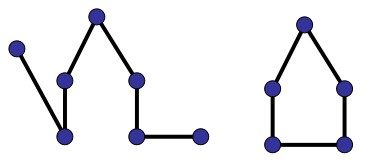
\includegraphics[width=\textwidth]{l3/S001.jpg}
		\caption{Линии}
	\end{subfigure}
	\begin{subfigure}[b]{0.3\textwidth}
		\centering
		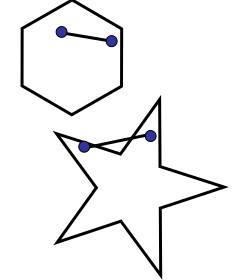
\includegraphics[width=\textwidth]{l3/S002.jpg}
		\caption{Многоугольники}
	\end{subfigure}
	\caption{Графические примитивы}
\end{figure}
\paragraph{Lines \& Polylines. } Линия, нарисованная по заданным точкам. Соединенные конечные точки дают \textbf{замкнутую полилинию} или \textbf{полигон}
\paragraph{Выпуклый и вогнутый многоугольники}
\textbf{Выпуклый}: Для каждой пары точек в многоугольнике линия между ними полностью содержится в многоугольнике.\\
\textbf{Вогнутый}: Не выпуклый: произвольные две точки соединенные в многоугольнике линией не полностью содержавшаяся в многоугольнике

\paragraph{Окружность. }  Состоит из всех точек равноудаленных от единой точки – центра окружности. $r^2 = x^2 + y^2$. Окружность может быть аппроксимирована как полигон с множеством сторон.
\screenshot{width=\textwidth}{l3/S003.jpg}{Аппроксимация окружности}

\paragraph{Эллипс. } Окружность, промасштабированная вдоль осей $x$ или $y$.
\screenshot{width=\textwidth}{l3/S004.jpg}{Эллипс}

\subsection{Введение в вычислительную геометрию}
\subsubsection{Аффинные и проективные преобразования на 	плоскости и в 3D-пространстве}
\textbf{Affinis} (лат.) – смежный, соседний, родственный
Признаки:
\begin{itemize}
	\item прямые линии остаются прямыми
	\item параллельные - параллельными
\end{itemize}
Примеры:
\begin{itemize}
	\item подобие (сохраняются углы)
	\item сжатие/растяжение (без подобия)
	\item движение (перенос и вращение – ортогональные преобразования 1-го рода)
\end{itemize}

\textbf{А.П.} можно определить с помощью невырожденных линейных преобразований точек пространства. \textbf{А.П.} - это подмножество проективных преобразований (П.П.).
При \textbf{П.П.} параллельность может нарушаться. Сохранение
параллельности является «границей», при нарушении которой \textbf{А.П.} превращаются в П.П.

\subsubsection{Элементарные преобразования на плоскости}
Универсальная, но чаще всего неудобная форма записи:
$$
\begin{cases}
	x'=ax_1+by_1+c_1\\
	y'=ax_2+by_2+c_2
\end{cases}; \ 
\begin{vmatrix}
	a_1 & b_1 \\
	a_2 & b_2
\end{vmatrix} \ne 0
$$
Более пригодная форма для использования в алгоритмах визуализации «собирается» из элементарных преобразований:
\begin{itemize}
	\item поворот вокруг начала координат на угол $\phi$
	\item растяжение (сжатие) вдоль координатных осей
	\item отражение относительно координатных осей
	\item перенос
\end{itemize}

Теоремы аффинной геометрии идентичны теоремам евклидовой геометрии, в которой важными понятиями являются параллельность и соотношение между параллельными линиями.

Аффинные преобразования формируют удобную подсистему билинейных преобразований, так как произведение двух аффинных преобразований также является аффинным. Преобразования связаны с некоторыми изменениями объекта.

Базовыми являются следующие преобразования:
\begin{itemize}
	\item Перенос (Move/Translation);
	\item Поворот (Rotate);
	\item Масштабирование (Scale);
	\item Отражение (Reflect);
	\item Сдвиг по одной из координат (Shear).
\end{itemize}
Преобразование объекта = преобразование всех его точек; преобразование полигона = преобразование всех его вершин

\subsubsection{Умножение матрицы на вектор}
$$
M_v = \begin{bmatrix}
M_{11} & M_{12} & M_{13}\\
M_{21} & M_{22} & M_{23}\\
M_{31} & M_{32} & M_{33}
\end{bmatrix} \cdot \begin{bmatrix}
v_x \\ v_y \\ x_z
\end{bmatrix} = \begin{bmatrix}
a \\ b \\ c
\end{bmatrix}
$$
Линейное преобразование вектора преобразует один вектор в другой и сохраняет линейные комбинации
Любое линейное преобразование м.б. представлено с
помощью матриц:
\begin{itemize}
	\item Масштабирование (scaling)
	\item Поворот (rotation)
	\item Перенос (translation)
\end{itemize}

\subsubsection{О порядке перемножения матриц и векторов}
\begin{enumerate}
	\item $b = a \cdot M$\\
	Неудобно: Не совпадает расположение элементов в  матрице и коэффициентов в записи системы уравнений.\\
	Удобно: Совпадают порядок перемножения матриц и порядок выполнения суперпозиции преобразований: \\
	$P_4(P_3(P_2(P_1))) \rightarrow M_1 \cdot M_2 \cdot M_3 \cdot M_4$
	\item $b^T = M^T \cdot a^T$\\
	Порядок перемножения матриц обратен	порядку преобразований в записи их суперпозиции, матрицы транспонированы по отношению к их записи в (1):\\
	$P_4(P_3(P_2(P_1))) \rightarrow M_4^T \cdot M_3^T \cdot M_2^T \cdot M_1^T$\\
	Удобно: Совпадает расположение элементов в матрице и коэффициентов в записи систем
\end{enumerate}

Примечания:
\begin{enumerate}
	\item Строго говоря, $М$ следовало бы считать $М^T$ ввиду запись матрицы по строкам, однако во избежание нагромождения символов, считаем здесь и далее запись матрицы по столбцам не транспонированной
	\item В математической литературе чаще используется порядок перемножения (1)
	\item В литературе по API OpenGL частенько используется порядок перемножения (2)
	\item «Удобства» и «неудобства» относительны (многое зависит от контекста алгоритма) 
\end{enumerate}

\subsection{2D перенос (Translation)}
\screenshot{width=9cm}{l3/S005.jpg}{Перенос}
$$
v'=v+t, \textrm{где} \ 
v=\begin{bmatrix} x \\ y \end{bmatrix}
v'=\begin{bmatrix} x' \\ y' \end{bmatrix}
t=\begin{bmatrix} \delta x \\ \delta y \end{bmatrix}
$$
$$
\begin{cases}
	x'=x+\delta x\\
	y'=y+\delta y
\end{cases}
$$
Длины и углы сохраняются.

\subsection{2D масштабирование}
\begin{figure}[h]
	\centering
	\begin{subfigure}[b]{0.4\textwidth}
		\centering
		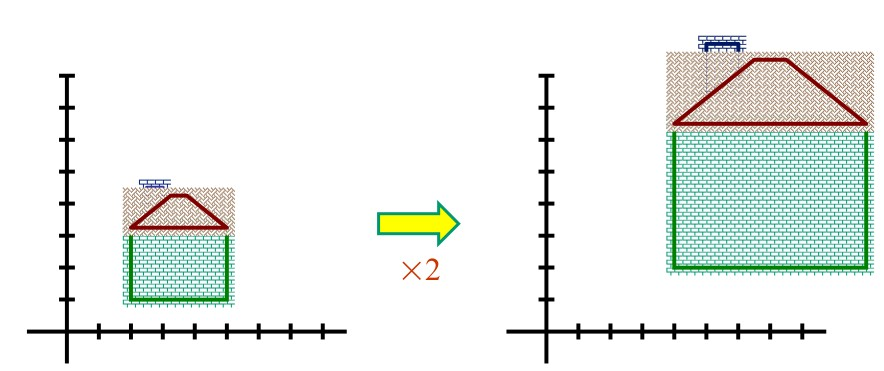
\includegraphics[width=\textwidth]{l3/S006.jpg}
		\caption{Однородное}
	\end{subfigure}
	\begin{subfigure}[b]{0.4\textwidth}
		\centering
		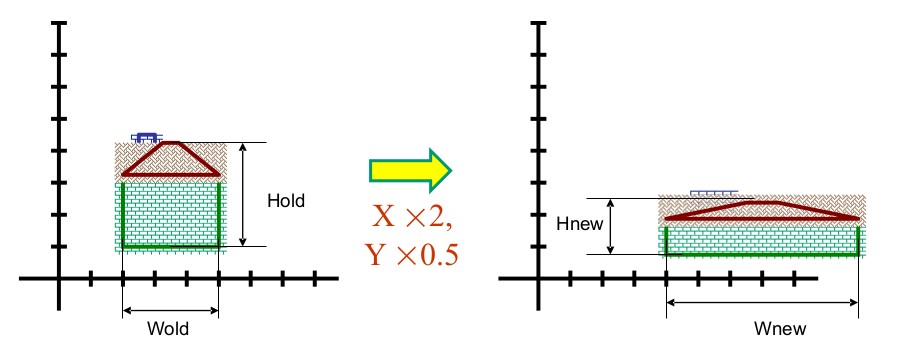
\includegraphics[width=\textwidth]{l3/S007.jpg}
		\caption{Неоднородное}
	\end{subfigure}
	\caption{Масштабирование}
\end{figure}
\textbf{Масштабирование} координаты означает умножать каждый из ее компонентов на скаляр. \textbf{однородное} масштабирование означает, что этот скаляр - одинаковый для всех компонентов. Соответственно, при \textbf{неоднородном} скаляры различны для каждого компонента.
$$
v' = S \cdot v; \textrm{где} \ v=\begin{bmatrix} x \\ y \end{bmatrix}, v'=\begin{bmatrix} x' \\ y' \end{bmatrix}
$$
$$
\begin{cases}
	x'=s_x x\\
	y'=s_y y
\end{cases}; \
S = \begin{bmatrix}
	s_x & 0 \\
	0 & s_y
\end{bmatrix}
$$
В таком случае длины и углы не сохраняются. Кроме того, имеется побочный эффект - на картинке дом перемещается относительно центра

\subsection{2D поворот}
\screenshot{width=6cm}{l3/S008.jpg}{Поворот}
Выразим $x$, $y$, $x'$, $y'$ в полярных координатах:
$$
\begin{cases}
	x = r\cos{\phi}\\
	y = r\sin{\phi}
\end{cases}; \ 
\begin{cases}
	x' = r\cos{\phi + \theta}\\
	y' = r\sin{\phi + \theta}
\end{cases}
$$
Раскроем последнюю систему:
$$
\begin{cases}
	x' = r\cos{\phi}\cos{\theta} - r\sin{\phi}\sin{\theta}\\
	y' = r\sin{\phi}\cos{\theta} + r\cos{\phi}\sin{\theta}
\end{cases}
$$
После замены получается следующая система:
$$
\begin{cases}
	x'=x\cos{\theta} - y\sin{\theta}\\
	y'=x\sin{\theta} + y\cos{\theta}
\end{cases}
$$
Это легко выразить в матричной форме:
$$
\begin{bmatrix} x' \\ y' \end{bmatrix} = \begin{bmatrix}
	\cos{\theta} & -\sin{\theta} \\
	\sin{\theta} & \cos{\theta}
\end{bmatrix} \cdot \begin{bmatrix} x \\ y \end{bmatrix}
$$

Если что объект не расположен в центре СК а его нужно масштабировать и вращать, переместитесь в НК, масштабируйте и/или вращайте его в местной системе координат, затем переместите объект обратно. Эта последовательность предлагает потребность составить последовательные (составные) преобразования.

\subsection{Однородные координаты}
\textbf{Однородные координаты} - это математический механизм, связанный с определением положения точек в пространстве. Привычный аппарат декартовых координат, не подходит для решения некоторых важных задач в силу следующих соображений:
\begin{itemize}
	\item В декартовых координатах невозможно описать бесконечно удаленную точку. А многие математические и геометрические концепции значительно упрощаются, если в них используется понятие бесконечности. Например, "бесконечно удаленный источник света".
	\item С точки зрения алгебраических операций, декартовы координаты не позволяют провести различия межу точками и векторами в пространстве. Действительно, $(1,2,5)$ - это направление или точка?
	\item Невозможно использовать унифицированный механизм работы с матрицами для выражения преобразований точек. С помощью матриц $3 \times 3$ можно описать вращение и масштабирование, однако описать смещение $(x=x+a)$ нельзя.
	\item Аналогично, декартовы координаты не позволяют использовать матричную запись для задания перспективного преобразования (проекции) точек.
\end{itemize}
Для решения этих проблем используются однородные координаты.

\screenshot{width=9cm}{l3/S009.jpg}{Однородные координаты}
$P_{2d}$ - пересечение линии, определённой $P_h$ с плоскостью $w=1$.
Композицию преобразований трудно выразить, пока перенос не выражен как матричное умножение. Но, если мы выразим точки в однородных координатах, то все три преобразования можно реализовать с помощью умножений.

Однородные координаты были введены в геометрии и впоследствии использованы в графике. С однородными координатами и преобразованиями над ними работают многие пакеты графических подпрограмм и некоторые дисплейные процессоры.

В одних случаях эти координаты используются прикладной программой непосредственно при задании параметров для графического пакета, в других — применяются лишь внутри самого пакета и недоступны для программиста.
Теперь матрицы преобразований выглядят так:
$$
R(\theta)=\begin{bmatrix}
	\cos{\theta} & -\sin{\theta} & 0 \\
	\sin{\theta} & \cos{\theta} & 0 \\
	0 & 0 & 1
\end{bmatrix}; \ 
S(a,b) = \begin{bmatrix}
	a & 0 & 0 \\
	0 & b & 0 \\
	0 & 0 & 1
\end{bmatrix}; \
T(x,y) = \begin{bmatrix}
	1 & 0 & x \\
	0 & 1 & y \\
	0 & 0 & 1
\end{bmatrix}
$$
Перенос работает следующим образом:
$$
\begin{bmatrix}
	1 & 0 & a \\
	0 & 1 & b \\
	0 & 0 & 1
\end{bmatrix} \cdot \begin{bmatrix}
	x \\ y \\ 1
\end{bmatrix} = \begin{bmatrix}
	 x + a \\ y + b \\ 1
\end{bmatrix}
$$

\subsection{Отражение}
\begin{figure}[h]
	\centering
	\begin{subfigure}[b]{0.2\textwidth}
		\centering
		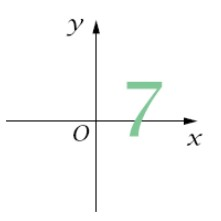
\includegraphics[width=\textwidth]{l3/S010.jpg}
		\caption{Исходный рисунок}
	\end{subfigure}
	\begin{subfigure}[b]{0.2\textwidth}
		\centering
		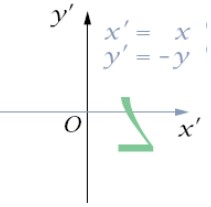
\includegraphics[width=\textwidth]{l3/S011.jpg}
		\caption{Вдоль $x$}
	\end{subfigure}
	\begin{subfigure}[b]{0.2\textwidth}
		\centering
		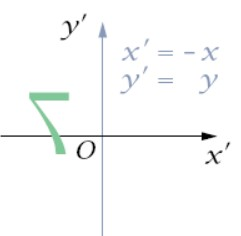
\includegraphics[width=\textwidth]{l3/S012.jpg}
		\caption{Вдоль $y$}
	\end{subfigure}
	\begin{subfigure}[b]{0.2\textwidth}
		\centering
		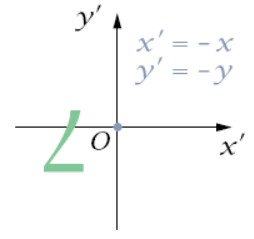
\includegraphics[width=\textwidth]{l3/S013.jpg}
		\caption{Вдоль обоих}
	\end{subfigure}
	\caption{Отражение}
\end{figure}
$$
\begin{bmatrix}
	x'_h \\ y'_h \\ h
\end{bmatrix} = \begin{bmatrix}
	1 & 0 & 0 \\
	0 & -1 & 0 \\
	0 & 0 & 1
\end{bmatrix} \cdot \begin{bmatrix}
	x_h \\ y_h \\ z_h
\end{bmatrix}
$$
Соответственно, матрица отражения вдоль x: 
$$
\begin{bmatrix}
	1 & 0 & 0 \\
	0 & -1 & 0 \\
	0 & 0 & 1
\end{bmatrix}
$$
Для отражения вдоль оси y или обеих осей используются следующие матрицы:
$$
\begin{bmatrix}
	-1 & 0 & 0 \\
	0 & 1 & 0 \\
	0 & 0 & 1
\end{bmatrix}; \ 
\begin{bmatrix}
	-1 & 0 & 0 \\
	0 & -1 & 0 \\
	0 & 0 & 1
\end{bmatrix}
$$

\subsection{Смещение (Shear)}
\begin{figure}[h]
	\centering
	\begin{subfigure}[b]{0.3\textwidth}
		\centering
		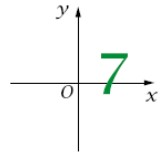
\includegraphics[width=\textwidth]{l3/S014.jpg}
		\caption{Исходный рисунок}
	\end{subfigure}
	\begin{subfigure}[b]{0.3\textwidth}
		\centering
		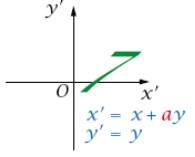
\includegraphics[width=\textwidth]{l3/S015.jpg}
		\caption{Вдоль $x$}
	\end{subfigure}
	\begin{subfigure}[b]{0.3\textwidth}
		\centering
		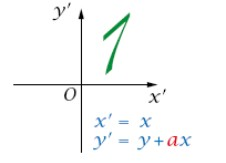
\includegraphics[width=\textwidth]{l3/S016.jpg}
		\caption{Вдоль $y$}
	\end{subfigure}
	\caption{Смещение}
\end{figure}
Матрицы смещения вдоль $x$ и $y$:
$$
\begin{bmatrix}
	1 & 0 & 0 \\
	a & 1 & 0 \\
	0 & 0 & 1
\end{bmatrix}; \ 
\begin{bmatrix}
	1 & a & 0 \\
	0 & 1 & 0 \\
	0 & 0 & 1
\end{bmatrix}
$$

\subsection{Порядок выполнения преобразований}
\screenshot{width=12cm}{l3/S017.jpg}{Некоммутативность}
Важно, что преобразования не коммутативны. 

\subsection{Создание преобразований}
\screenshot{width=12cm}{l3/S018.jpg}{Композиция преобразований}
Для получения нужного результата в данном случае нужно применить два преобразования подряд:
$$
p'=R(z,-90^\circ)p; \ p''=T(2,3,0)p' \ \rightarrow \ p''=T(2,3,0)R(z,90^\circ)p = TRp
$$

\subsubsection{Поворот вокруг произвольной точки $O$}
$$
C(O, \theta) = T(-O_x, -O_y)R(\theta)T(O_x, O_y)
$$

\subsubsection{Общий подход к композиции преобразований}
\begin{itemize}
	\item Преобразование геометрии объектов в такую систему координат, где операция становится более простой;
	\item Выполните операцию;
	\item Преобразуйте геометрию объектов сцены назад к первоначальной системе координат
\end{itemize}

\section{3D преобразования}
\subsection{Системы координат, используемые в графике}
\definition{Координаты экрана} - физическое местоположение на определённом устройстве вывода (отображения). Определяют местоположение пикселей.
\begin{itemize}
	\item Изменения трудны для прикладной программы
	\item Приводит к зависимому от устройства кода
\end{itemize}
\screenshot{width=8cm}{l4/S001.jpg}{Коррдинаты экрана}

\definition{Координаты окна} - экранные координаты относительно центра окна.
Система GUI дает приложению позицию на экране; оконная система преобразует координаты окна в экранные координаты
\screenshot{width=8cm}{l4/S002.jpg}{Координаты окна}

\definition{Нормализованные координаты устройства (NDC)} - независимая от устройства абстракция окна экрана.
\begin{itemize}
	\item Абстракция координат
	\item Значение координат - вещественные числа с плавающей запятой от 0 до 1
\end{itemize}
\screenshot{width=8cm}{l4/S003.jpg}{Нормализованные координаты}

\definition{Мировые координаты} - родовая система координат, которую может использовать любое приложение, чтобы определить объекты для показа
\begin{itemize}
	\item Приложение должно быть в состоянии определить объекты в форму, естественную для области. Например, от $0$ до $10^4$  км для карты России
	\item Мировые координаты - 2D или 3D значение с плавающей точкой, которые могут представить местоположения и размеры объекта, который будет показан.
\end{itemize}

\subsection{Преобразования в мировом пространстве}
Шаги преобразования:
\begin{itemize}
	\item Объект в МК
	\item Окно переносится в начало координат
	\item Масштабирование окна под размер поля вывода (нормализация в uv)
	\item Перенос в окончательную позицию
\end{itemize}
\screenshot{width=12cm}{l4/S004.jpg}{Преобразования координат}

\subsection{Использование нормализованных координат}
Трехмерная точка в трехмерном пространстве $P(x,y,z)$ представится четырёхмерным вектором
$\begin{bmatrix}
x & y & z & 1
\end{bmatrix}$
 или 
$\begin{bmatrix}
X & Y & Z & W
\end{bmatrix}$\\
\newpage
Преобразования из однородных координат описываются соотношениями:
$$\begin{bmatrix} X & Y & Z & W \end{bmatrix} = 
\begin{bmatrix} x & y & z & 1 \end{bmatrix} \cdot T$$
$$\begin{bmatrix} x' & y' & z' & 1 \end{bmatrix} = 
\begin{bmatrix} \dfrac{X}{W} & \dfrac{Y}{W} & \dfrac{Z}{W} & 1 \end{bmatrix}
$$
Где T - некоторая матрица преобразования. Обобщенная матрица преобразования $4\times4$ для трехмерных координат имеет вид:
$$ T = \begin{bmatrix}
a & b & c & p\\
d & e & f & q\\
h & i & j & r\\
I & m & n & s
\end{bmatrix} $$
Эта матрица может быть представлена в виде четырёх отдельных частей:
$$
\begin{array}{c|c}
\lbrack 3 \times 3 \rbrack & \lbrack 3 \times 1 \rbrack \\ 
\hline
\lbrack 1 \times 3 \rbrack & \lbrack 1 \times 1 \rbrack
\end{array}
$$
Матрица $3 \times 3$ осуществляет линейное преобразование в виде изменения масштаба, сдвига и вращения. Матрица-строка $1 \times 3 $ производит перенос, а матрица-столбец $3 \times 1$ - преобразование в перспективе. Последний скалярный элемент выполняет общее изменение масштаба.

Важно, что 3D-преобразования \textbf{некоммутативны}, т.е. изменения порядка применения преобразований может привести к изменению результата
\screenshot{width=9cm}{l4/S008.jpg}{Коммутативность 3D-преобразований}
\subsubsection{Перенос}
$$
\begin{bmatrix} x' \\ y' \\ z' \\ 1 \end{bmatrix} = 
\begin{bmatrix}
	1 & 0 & 0 & t_x \\
	0 & 1 & 0 & t_y \\
	0 & 0 & 1 & t_z \\
	0 & 0 & 0 & 1
\end{bmatrix}
\cdot
\begin{bmatrix} x \\ y \\ z \\ 1 \end{bmatrix}
$$
\screenshot{width=12cm}{l4/S005.jpg}{Перенос}

\subsubsection{Масштабирование}
$$
\begin{bmatrix} x' \\ y' \\ z' \\ 1 \end{bmatrix} = 
\begin{bmatrix}
s_x & 0 & 0 & 0 \\
0 & s_y & 0 & 0 \\
0 & 0 & s_z & 0 \\
0 & 0 & 0 & 1
\end{bmatrix}
\cdot
\begin{bmatrix} x \\ y \\ z \\ 1 \end{bmatrix}
$$
\screenshot{width=12cm}{l4/S006.jpg}{Масштабирование}

\subsubsection{Повороты}
\paragraph{Поворот по оси z}
$$
\begin{bmatrix} x' \\ y' \\ z' \\ 1 \end{bmatrix} = 
\begin{bmatrix}
\cos(\theta) & -\sin(\theta) & 0 & 0 \\
\sin(\theta) & \cos(\theta) & 0 & 0 \\
0 & 0 & 1 & 0 \\
0 & 0 & 0 & 1
\end{bmatrix}
\cdot
\begin{bmatrix} x \\ y \\ z \\ 1 \end{bmatrix}
$$
\screenshot{width=12cm}{l4/S007.jpg}{Поворот по оси z}

\paragraph{Поворот по оси x}
$$
\begin{bmatrix} x' \\ y' \\ z' \\ 1 \end{bmatrix} = 
\begin{bmatrix}
1 & 0 & 0 & 0 \\
0 & \cos(\theta) & -\sin(\theta) & 0 \\
0 & \sin(\theta) & \cos(\theta) & 0 \\
0 & 0 & 0 & 1
\end{bmatrix}
\cdot
\begin{bmatrix} x \\ y \\ z \\ 1 \end{bmatrix}
$$

\paragraph{Поворот по оси y}
$$
\begin{bmatrix} x' \\ y' \\ z' \\ 1 \end{bmatrix} = 
\begin{bmatrix}
\cos(\theta) & 0 & \sin(\theta) & 0 \\
0 & 1 & 0 & 0 \\
-\sin(\theta) & 0 & \cos(\theta) & 0 \\
0 & 0 & 0 & 1
\end{bmatrix}
\cdot
\begin{bmatrix} x \\ y \\ z \\ 1 \end{bmatrix}
$$

\subsubsection{3D положительное вращение}
\begin{tabular}{| c | c |}
	\hline
	\textbf{Ось вращения} & \textbf{Положительным будет направление поворота} \\
	\hline
	$x$ & от $y$ к $z$\\
	\hline
	$y$ & от $z$ к $x$\\
	\hline
	$z$ & от $x$ к $y$\\
	\hline
\end{tabular}

\subsection{Формирование матрицы преобразования}
\subsubsection{Примеры преобразований}
\texttt{glTranslate} и \texttt{glRotate} всегда относятся к текущему состоянию матрицы. Например, если вы вызываете \texttt{glTranslate}, вы переводите из текущей "позиции" матрицы, а не из начала координат. Но если вы хотите начать с начала координат, когда вы вызываете \texttt{glLoadIdentity}(), а затем вы можете взять \texttt{glTranslate} из матрицы, которая теперь находится в начале координат, или \texttt{glRotate} из матрицы, которая теперь ориентирована по умолчанию.

\begin{lstlisting}[language=C]
mat4 m = Identity();
\end{lstlisting}
$$
m = \begin{pmatrix}
1 & 0 & 0 & 0\\
0 & 1 & 0 & 0\\
0 & 0 & 1 & 0\\
0 & 0 & 0 & 1
\end{pmatrix}
$$
\begin{lstlisting}[language=C]
mat4 m = Identity();
mat4 t = Translate(3,6,4);
m = m * t;
\end{lstlisting}
$$\textrm{Identity Matrix} \cdot \textrm{Translation Matrix} = \textrm{CTM Matrix}$$
$$
\begin{pmatrix}
1 & 0 & 0 & 0\\
0 & 1 & 0 & 0\\
0 & 0 & 1 & 0\\
0 & 0 & 0 & 1
\end{pmatrix}
\cdot
\begin{pmatrix}
1 & 0 & 0 & 3\\
0 & 1 & 0 & 6\\
0 & 0 & 1 & 4\\
0 & 0 & 0 & 1
\end{pmatrix}
=
\begin{pmatrix}
1 & 0 & 0 & 3\\
0 & 1 & 0 & 6\\
0 & 0 & 1 & 4\\
0 & 0 & 0 & 1
\end{pmatrix}
$$
\begin{lstlisting}[language=C]
mat4 m = Identity();
mat4 t = Scale(1,2,3);
m = m * s;
\end{lstlisting}
$$\textrm{Identity Matrix} \cdot \textrm{Scaling Matrix} = \textrm{CTM Matrix}$$
$$
\begin{pmatrix}
1 & 0 & 0 & 0\\
0 & 1 & 0 & 0\\
0 & 0 & 1 & 0\\
0 & 0 & 0 & 1
\end{pmatrix}
\cdot
\begin{pmatrix}
1 & 0 & 0 & 0\\
0 & 2 & 0 & 0\\
0 & 0 & 3 & 0\\
0 & 0 & 0 & 1
\end{pmatrix}
=
\begin{pmatrix}
1 & 0 & 0 & 0\\
0 & 2 & 0 & 0\\
0 & 0 & 3 & 0\\
0 & 0 & 0 & 1
\end{pmatrix}
$$

\begin{lstlisting}[language=C]
mat4 m = Identity();
mat4 s = Scale(1,2,3);
mat4 t = Translate(3,6,4);
m = m * s * s;
\end{lstlisting}
$$\textrm{Identity Matrix} \cdot \textrm{Scaling Matrix} \cdot \textrm{Translate Matrix} = \textrm{Final CTM}$$
$$
\begin{pmatrix}
1 & 0 & 0 & 0\\
0 & 1 & 0 & 0\\
0 & 0 & 1 & 0\\
0 & 0 & 0 & 1
\end{pmatrix}
\cdot
\begin{pmatrix}
1 & 0 & 0 & 0\\
0 & 2 & 0 & 0\\
0 & 0 & 3 & 0\\
0 & 0 & 0 & 1
\end{pmatrix}
\cdot
\begin{pmatrix}
1 & 0 & 0 & 3\\
0 & 1 & 0 & 6\\
0 & 0 & 1 & 4\\
0 & 0 & 0 & 1
\end{pmatrix}
=
\begin{pmatrix}
1 & 0 & 0 & 3\\
0 & 2 & 0 & 12\\
0 & 0 & 3 & 12\\
0 & 0 & 0 & 1
\end{pmatrix}
$$

\subsubsection{Применение преобразований в OpenGL}
\paragraph{В приложении. }
Массив точек загружается в VBO; вызывается \texttt{glDrawArrays()}. CTM, сформированная в приложении, подается в вершинный шейдер, например, следующим образом:
\begin{lstlisting}[language=C]
matrix_loc = glGetUniformLocation(program, "model_view");
glUniformMatrix4fv(matrix_loc, 1, GL_TRUE, m);
\end{lstlisting}

\paragraph{В вершинном шейдере.} Каждая вершина объекта умножается на CTM, чтобы получить позицию вершины
\begin{lstlisting}[language=C]
in vec4 vPosition;
uniform mat4 model_view;

void main(){
	gl_Position = model_view * vPosition;
}

\end{lstlisting}

\subsection{Пример 3D преобразований}
\setcounter{stepcounter}{1}
\screenshot{width=9cm}{l4/S009.jpg}{Целевое преобразование}

\steppar Перенос $P_1$ в начало координат
$$T(-x_1, -y_1, -z_1) = \begin{vmatrix}
1 & 0 & 0 & -x_1\\
0 & 1 & 0 & -y_1\\
0 & 0 & 1 & -z_1\\
0 & 0 & 0 & 1
\end{vmatrix} $$
\screenshot{width=9cm}{l4/S010.jpg}{После первого шага}

\steppar Поворот вокруг оси $Y_1$, т.е., чтобы $P_1 P_2$ переместилась в плоскость $0YZ$
$$\theta' = - (90^\circ - \theta)$$
$$\cos{\theta} = \dfrac{z'_2}{D_1}; sin{\theta} = - \dfrac{x'_2}{D_1}$$
$$D_1=\sqrt{(z'_2)^2 + (x'_2)^2}; P''_2 = R_y (\theta - 90^\circ)P'_2$$
\screenshot{width=6cm}{l4/S011.jpg}{После второго шага}

\steppar Поворот вокруг оси $X$, чтобы $P_1 P_2$ совместилась с осью Z
$$\cos{\psi} = \dfrac{z''_2}{D_2}; \sin{\psi} = \dfrac{y''_2}{D_2}$$
$$D_2 = |P''_1 P''_2| = |P_1 P_2| = \sqrt{(x_2-x_1)^2 + (y_2-y_1)^2 + (z_2-z_1)^2}$$
$$P''_2=R_x(\psi)R''_2=R_x(\psi)R_y(\theta-90^\circ)P'_2$$
\screenshot{width=6cm}{l4/S012.jpg}{После третьего шага}

\steppar Поворот вокруг оси $Z$. Поместить $P_3$ в плоскость $YOZ$
$$P'''_3=|\begin{matrix} X'''_3 & Y'''_3 & Z'''_3 \end{matrix}|T = R_X(\phi) R_Y(\theta-90^\circ) T(-x_1, -y_1, -z_1) P_3
$$
\screenshot{width=6cm}{l4/S013.jpg}{После четвертого шага}

Полная матрица будет выглядеть так:
$$R_Z (\alpha) R_X (\phi) R_Y (\theta-90) 
T(-x_1,-y_1,-z_1)P_3$$

\subsection{Трехмерное вращение вокруг произвольной оси}
Для этого можно использовать \textbf{теорему Эйлера}: любая последовательность вращений = одно вращение вокруг некоторой оси.\\
Наш подход:
\begin{enumerate}
	\item Хотим вращать $\beta$ вокруг оси $u$ через НК и произвольной точки
	\item Используем два вращения, чтобы выравнять $u$ и ось $X$
	\item Делаем $x$-поворот через угол $\beta$
	\item Два обратные предыдущих вращения, чтобы девыровнять $u$ и ось $X$
\end{enumerate}

$$ R_u(\beta) = R_y(-\theta)R_z(\phi)R_x(\beta)R_z(-\phi)R_y(\theta)$$
\screenshot{width=9cm}{l4/S014.jpg}{Вращение вокруг произвольной оси}

\subsection{Примеры решения наиболее важных задач}
\subsubsection{Поворот вокруг точки на плоскости}\label{pointturn}
Построить матрицу поворота на угол $\phi$ вокруг точки $A(a,b)$ на плоскости
\setcounter{stepcounter}{1}
\steppar Перенос на вектор $-A=(-a, -b)$ для совмещения оси поворота с началом координат
$$ T_{-A} = \begin{pmatrix}
1 & 0 & 0\\
0 & 1 & 0\\
-a & -b & 1
\end{pmatrix} $$
\steppar Поворот на угол $\phi$
$$ R_\phi = \begin{pmatrix}
\cos{\phi} & \sin{\phi} & 0\\
-\sin{\phi} & \cos{\phi} & 0\\
0 & 0 & 1
\end{pmatrix} $$
\steppar Перенос на вектор $A=(a,b)$ для возвращения оси поворота в прежнее положение
$$ T_{A} = \begin{pmatrix}
1 & 0 & 0\\
0 & 1 & 0\\
a & b & 1
\end{pmatrix} $$
\steppar Формирование матрицы $M$ итогового преобразования
$$ M=T_{-A} R_\phi T_A $$
\subsubsection{Отражение относительно прямой}
Построить матрицу отражения плоского полигона \{$A_i$\} относительно прямой $I$, проходящей на плоскости через начало координат под углом $\phi$ к оси абсцисс.

\screenshot{width=8cm}{l4/S015.jpg}{Отражение относительно прямой}

\setcounter{stepcounter}{1}
\steppar Поворот оси $X$ до совпадения с осью отражения $I$
$$ R_\phi = \begin{pmatrix}
\cos{\phi} &- \sin{\phi} & 0\\
\sin{\phi} & \cos{\phi} & 0\\
0 & 0 & 1
\end{pmatrix} $$

\steppar Отражение относительно оси $X$
$$ S_{X} = \begin{pmatrix}
1 & 0 & 0\\
0 & -1 & 0\\
0 & 0 & 1
\end{pmatrix} $$

\steppar Возврат системы координат в исходное состояния
$$ R_\phi^{-1} = \begin{pmatrix}
\cos{\phi} & \sin{\phi} & 0\\
-\sin{\phi} & \cos{\phi} & 0\\
0 & 0 & 1
\end{pmatrix} $$

\steppar Формирование матрицы итогового преобразования
$$M=R_\phi S_x R_\phi^{-1}$$

\steppar Преобразование координат каждой вершины полигона
$$A'_i = A_iM, i=1,2,...$$

\subsubsection{Поворот вокруг прямой в 3D-пространстве}
\setcounter{stepcounter}{1}
\screenshot{width=8cm}{l4/S016.jpg}{Вращение вокруг прямой в 3D-пространстве}

Построить матрицу поворота на угол $\phi$ вокруг прямой $L$ в 3D-пространстве, проходящей через точку $A=(a,b,c)$ и имеющей направляющий вектор $(l,m,m)$ с модулем, равным единице.

Решение похоже на рассмотренное в \ref{pointturn}, но здесь ось вращения задается в 3D-пространстве и ориентирована произвольно.

Матрицы переноса и возврата:
$$
T=\begin{bmatrix}
1 & 0 & 0 & 0\\
0 & 1 & 0 & 0\\
0 & 0 & 1 & 0\\
-a & -b & -c & 1
\end{bmatrix}; \quad
T^{-1} = \begin{bmatrix}
1 & 0 & 0 & 0\\
0 & 1 & 0 & 0\\
0 & 0 & 1 & 0\\
a & b & c & 1
\end{bmatrix}
$$
Пусть ось вращения, заданная в условии, будет осью $Z$ системы координат в новом положении, в которое мы её переведём двумя вращениями сначала вокруг оси $X$, потом вокруг новой оси $Y$ (после вращения вокруг этой оси нужно будет "вернутся обратно")\\
Зададим матрицы вращения:
$$
R_z = \begin{bmatrix}
\cos{\phi} & \sin{\phi} & 0 & 0\\
-\sin{\phi} & \cos{\phi} & 0 & 0\\
0 & 0 & 1 & 0\\
0 & 0 & 0 & 1
\end{bmatrix}; \
R_x = \begin{bmatrix}
1 & 0 & 0 & 0\\
0 & \frac{n}{d} & \frac{m}{d} & 0\\
0 & -\frac{m}{d} & \frac{n}{d} & 0\\
0 & 0 & 0 & 1
\end{bmatrix}; \ 
R_y = \begin{bmatrix}
d & 0 & l & 0\\
- & 1 & 0 & 0\\
-l & 0 & d & 0\\
0 & 0 & 0 & 1
\end{bmatrix}
$$
Где
$$d=\sqrt{m^2+n^2}; \ \sin{\psi} = \dfrac{m}{d}; \ \cos{\psi} = \dfrac{n}{d}$$

\begin{figure}[h]
	\centering
	\begin{subfigure}[b]{0.3\textwidth}
		\centering
		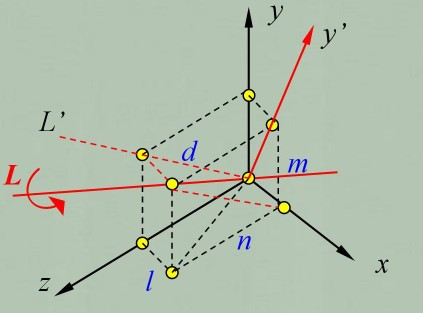
\includegraphics[width=\textwidth]{l4/S017.jpg}
		\caption{Матрица $R_z$}
	\end{subfigure}
	\begin{subfigure}[b]{0.3\textwidth}
		\centering
		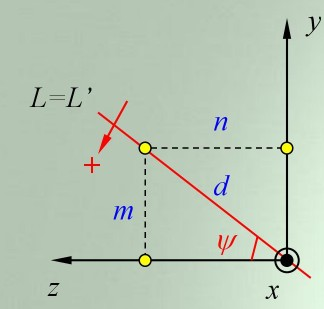
\includegraphics[width=\textwidth]{l4/S018.jpg}
		\caption{Матрица $R_x$}
	\end{subfigure}
	\begin{subfigure}[b]{0.3\textwidth}
		\centering
		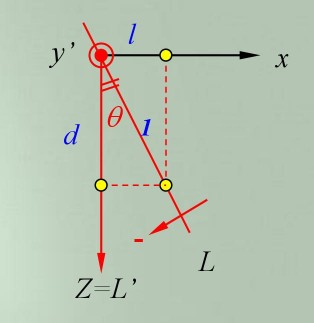
\includegraphics[width=\textwidth]{l4/S019.jpg}
		\caption{Матрица $R_z$}
	\end{subfigure}
	\caption{Матрицы поворота}
\end{figure}
Матрица итогового преобразования:
$$
M = T \cdot R_x \cdot R_y \cdot R_z \cdot R_y^{-1} \cdot R_x^{-1} \cdot T^{-1} = Q \cdot R_z \cdot Q^-1
$$
где
$$Q=T \cdot R_x \cdot R_y$$

\subsection{Граф сцены}
3D-сцены часто хранятся в направленном ациклическом графе (DAG), называемом \textbf{граф сцены}. Обычно такой граф состоит из:
\begin{itemize}
	\item Объекты (кубы, сферы, конусы, многогранники)
	\item Атрибуты (цвет, текстурные карты)
	\item Преобразования
\end{itemize}
\screenshot{width=\textwidth}{l4/S020.jpg}{Граф сцены}

Преобразования выступают такими же узлами в графе, как и объекты.
\begin{figure}[h]
	\centering
	\begin{subfigure}[b]{0.45\textwidth}
		\centering
		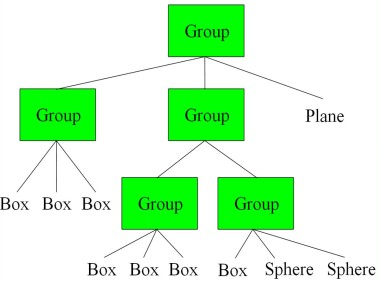
\includegraphics[width=\textwidth]{l4/S021.jpg}
		\caption{Без преобразований}
	\end{subfigure}
	\begin{subfigure}[b]{0.45\textwidth}
		\centering
		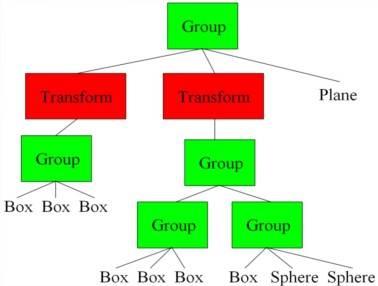
\includegraphics[width=\textwidth]{l4/S022.jpg}
		\caption{С преобразованиями}
	\end{subfigure}
	\caption{Преобразования}
\end{figure}

\section{Проецирование}
\subsection{История проецирования}
\subsection{Ранний вид проецирования}
\begin{figure}[h]
	\centering
	\begin{subfigure}[b]{0.45\textwidth}
		\centering
		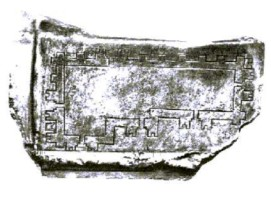
\includegraphics[width=\textwidth]{l5/S001.jpg}
		\caption{Месопотамия, XX в. до н.э.}
		\label{ancientproj1}
	\end{subfigure}
	\begin{subfigure}[b]{0.45\textwidth}
		\centering
		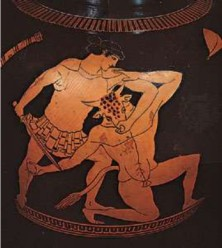
\includegraphics[width=\textwidth]{l5/S002.jpg}
		\caption{Греция, VI до н.э.}
		\label{ancientproj2}
	\end{subfigure}
	\caption{Раннее процирование}
\end{figure}
\ref{ancientproj1} - вид сверху (параллельный, особенно орфографический, проекционный) из Месопотамии (2150 г. до н.э.): самый ранний известный технический рисунок\\
\ref{ancientproj2} - греческая ваза конца VI века до нашей эры: показывает признаки попыток ракурса перспективы! Обратите внимание на относительные размеры бедер и нижних конечностей минотавра
\begin{figure}[h]
	\centering
	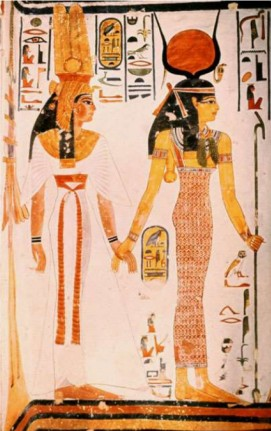
\includegraphics[width=6cm]{l5/S003.jpg}
	\caption{Египет, 1270 г. до н.э.}
	\label{ancientproj3}
\end{figure}
Древнеегипетское искусство:
\begin{itemize}
	\item Несколько точек обзора
	\item Параллельная проецирование (нет попытки изобразить перспективный ракурс)
\end{itemize}

\ref{ancientproj3} - Могила Нефертари, Фивы (19-й династии, - 1270 г. до н.э.). Королева, ведомая Исидой. Фреска.\\
Обратите внимание, как изображение тела подразумевает вид спереди, но ноги и голова подразумевают вид сбоку (ранний кубизм!)

\subsubsection{Эпоха Возрождения}
\begin{figure}[h]
	\centering
	\begin{subfigure}[b]{0.45\textwidth}
		\centering
		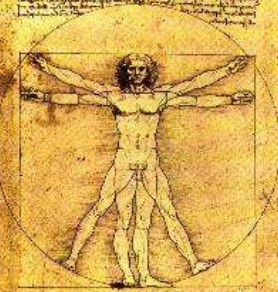
\includegraphics[width=\textwidth]{l5/S004.jpg}
	\end{subfigure}
	\begin{subfigure}[b]{0.45\textwidth}
		\centering
		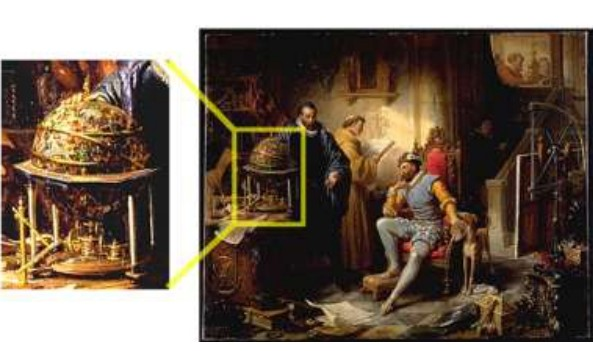
\includegraphics[width=\textwidth]{l5/S005.jpg}
	\end{subfigure}
	\caption{Проецирование в эпоху Возрождения}
\end{figure}

Начиная с ХIII века : новый акцент на важности индивидуальной точки зрения, мировой интерпретации, способности наблюдения (в частности природы: астрономии, анатомии и т.д.
\begin{itemize}
	\item Мазаччо, Донателло, Вселенная да Винчи в качестве часового механизма
\end{itemize}
Перестраивая вселенную более системно и механически:
\begin{itemize}
	\item Тихо Браге и Рудольф Ив Праге (деталь часового механизма), ок. 1585
	\item Коперник, Кеплер, Галилей, Ньютон ...: от земно-ориентированной до гелиоцентрической модели 	(механистической) вселенной, законы которой можно обнаружить и понять
\end{itemize}

\FloatBarrier
\subsubsection{Ранние попытки в перспективе}
\begin{figure}[h]
	\centering
	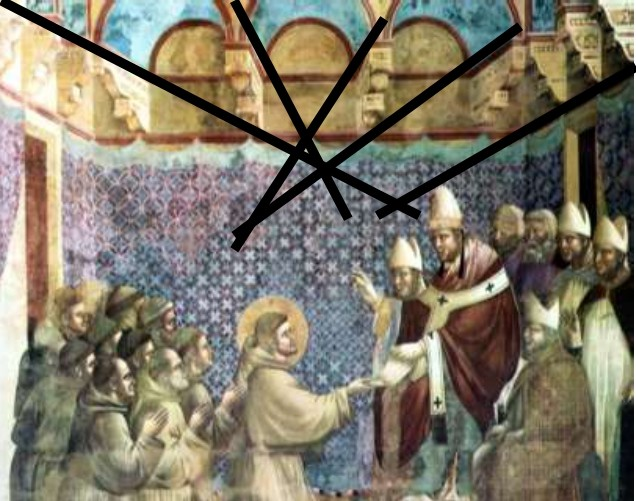
\includegraphics[width=9cm]{l5/S006.jpg}
	\caption{Джотто. Утверждение о францисканском правительстве}
	\label{renproj1}
\end{figure}
В искусстве более реалистично пытаться представить ЗD-пространство. Ранее работы вызывали ощущение пространства 3D, но не систематически. \ref{renproj1} - параллельные линии сходятся, но существует несколько точек схода

\subsubsection{Брунелесски и Вермеер}
\screenshot{width=9cm}{l5/S007.jpg}{Перспективный рисунок для церкви Санто Спирито во Флоренции}
Брунеллески изобрел систематический метод определения перспективной проекции (начало 1400-х годов). Он создал демонстрационные панели с особыми ограничениями просмотра для полной точности воспроизведения. \\
Вермеер и другие создали перспективные коробки, где изображение, просматриваемое через отверстие для обзора, имело правильную перспективу

Брунеллески определял точность своих картин, сделав отверстие в точке схода, и исследуя отражение в зеркале и сравнивая сходимость линии к реальной модели. 

Реализм его картин свидетельствует о том, что у Брунеллески был некоторый систематический метод определения перспективных проекций, хотя процедура, которую он использовал, никогда не была задокументирована. Его иллюзия вдохновила других художников на изучение линейной перспективы.

\FloatBarrier
\subsubsection{Camera Obscura}
\screenshot{width=9cm}{l5/S008.jpg}{Камера обскура}
Камера-обскура (лат. camera obscura — «тёмная комната»). Простейший вид устройства представляет собой светонепроницаемый ящик с отверстием в одной из стенок и экраном (матовым стеклом или тонкой белой бумагой) на противоположной стене. Лучи света, проходя сквозь малое отверстие (диаметр которого зависит от «фокусного расстояния» камеры, приблизительно 0,1—5 мм) создают перевёрнутое изображение на экране.

\begin{itemize}
	\item На основе камеры-обскуры были сделаны фотокамеры - фотографические аппараты без объектива
	\item Камера-обскура является частным случаем устройства с кодирующей апертурой.
	\item Ввиду отсутствия в камере-обскуре оптических элементов прямо воздействующих на свет (за исключением границы отверстия) она подходит для создания изображений в высокоэнергетических областях спектра
\end{itemize}
\begin{figure}[h]
	\centering
	\begin{subfigure}[b]{0.45\textwidth}
		\centering
		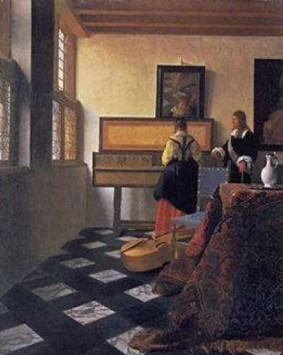
\includegraphics[width=\textwidth]{l5/S009.jpg}
		\caption{Картина}
	\end{subfigure}
	\begin{subfigure}[b]{0.45\textwidth}
		\centering
		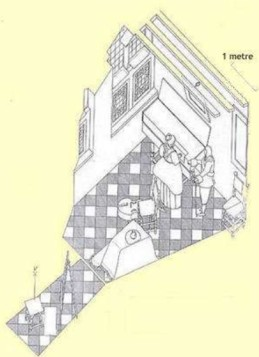
\includegraphics[width=\textwidth]{l5/S010.jpg}
		\caption{Реконструкция}
	\end{subfigure}
	\caption{Вермеер, урок музыки. 1662-1665}
\end{figure}
Вермеер, вероятно, использовал камеру-обскура, чтобы помочь формированию его шедевров; Также были созданы перспективные коробки, где у картины, когда она рассматривается через отверстие, была бы правильная перспектива.

\FloatBarrier
\subsubsection{Диего Веласкес, Пьерро дела Франческа}
\begin{figure}[h]
	\centering
	\begin{subfigure}[b]{0.45\textwidth}
		\centering
		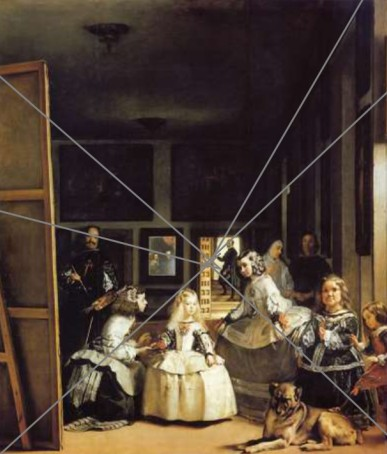
\includegraphics[width=\textwidth]{l5/S011.jpg}
		\caption{Диего Веласкес, 1656. Королевская семья}
		\label{renproj2}
	\end{subfigure}
	\begin{subfigure}[b]{0.45\textwidth}
		\centering
		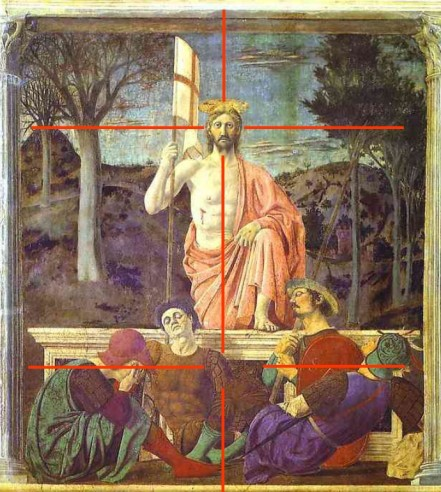
\includegraphics[width=\textwidth]{l5/S012.jpg}
		\caption{Пьеро дела Франческа (1460)}
		\label{renproj3}
	\end{subfigure}
	\caption{Влияние перспективы на на содержание}
\end{figure}
Точка зрения влияет на содержание и значение того, что отображается. \ref{renproj2} - Королевская пара находится в зеркале, но действительно ли это их изображение?\\
Анализ через компьютерную реконструкцию нарисованного места дает приговор: королевская пара в зеркале - отражение от холста на переднем плане, а не фактических людей.

Перспектива может использоваться, как способ управлять восприятием. \ref{renproj3} - Использование двух точек зрения концентрирует внимание зрителя поочередно на Христа и саркофаг.

\subsubsection{Правила линейной перспективы}
Идеи линейной перспективы:
\begin{itemize}
	\item Параллельные линии сходятся (по 1, 2 или 3 осям) к точке схода.
	\item Объекты, расположенные дальше, более искажены (т. е. меньше), чем ближе — тем больше
	\item Пример: перспективный куб
\end{itemize}
\FloatBarrier

\subsection{Геометрическое построение проекций}
\screenshot{width=9cm}{l5/S013.jpg}{Двухточечная проекция}

\subsubsection{Концептуальная модель}
\screenshot{width=\textwidth}{l5/S014.jpg}{Концептуальная модель процесса 2D вывода}

При визуализации двумерных изображений достаточно задать окно видимости в системе координат пользователя и порт отображения на экране дисплея, в котором будет выдаваться изображение из окна.

\screenshot{width=12cm}{l5/S015.jpg}{Модель и область видимости}

\screenshot{width=9cm}{l5/S018.jpg}{Угол обзора}

\begin{figure}[h]
	\centering
	\begin{subfigure}[b]{0.45\textwidth}
		\centering
		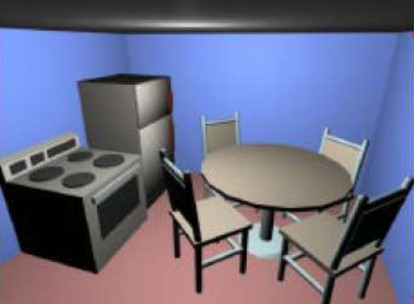
\includegraphics[width=\textwidth]{l5/S016.jpg}
		\caption{Правильно}
	\end{subfigure}
	\begin{subfigure}[b]{0.45\textwidth}
		\centering
		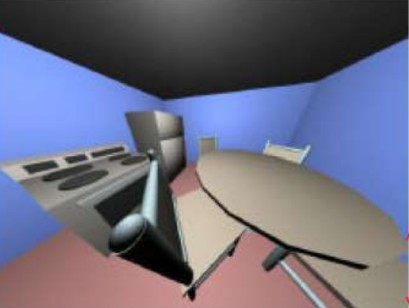
\includegraphics[width=\textwidth]{l5/S017.jpg}
		\caption{Неправильно}
	\end{subfigure}
	\caption{Настройка проекции}
\end{figure}

\FloatBarrier
\subsection{Ортографическое и перспективное проектирование}
\subsubsection{Камера}
\begin{figure}[h]
	\centering
	\begin{subfigure}[b]{0.45\textwidth}
		\centering
		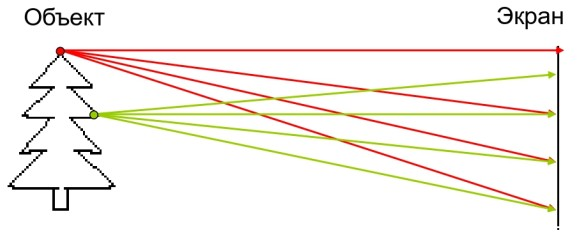
\includegraphics[width=\textwidth]{l5/S019.jpg}
		\caption{Бесполезная камера}
	\end{subfigure}
	\begin{subfigure}[b]{0.45\textwidth}
		\centering
		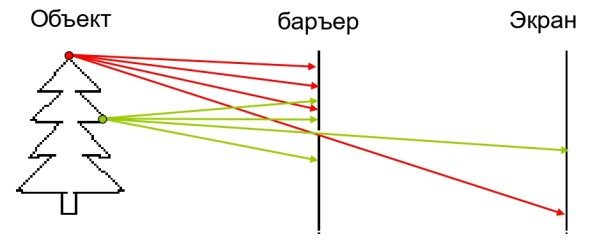
\includegraphics[width=\textwidth]{l5/S020.jpg}
		\caption{Камера-обскура}
	\end{subfigure}
	\caption{Камера}
\end{figure}
\paragraph{Простейшая камера.} Положим кусок пленки перед объектом. На каждую точку пленки падают лучи от всех точек объекта; получается бессмысленное изображение.
\paragraph{Камера-обскура.} Добавим преграду с отверстием, чтобы отсечь лишние лучи.
\begin{itemize}
	\item На каждую точку пленки падает один луч!
	\item Картинка должна быть четкой
	\item Отверстие в преграде называется \textbf{апертурой} или \textbf{диафрагмой}
\end{itemize}

\paragraph{Модель камеры-обскуры}
\screenshot{width=9cm}{l5/S021.jpg}{Камера-обскура}
\begin{itemize}
	\item В преграде отверстие размером в одну точку
	\item Все лучи проходят через одну точку
	\item Эта точка называется \textbf{центром проекции} (ЦП)
	\item Изображение формируется на \textbf{картинной плоскости}
	\item \textbf{Фокусным расстоянием} $f$ называется расстояние от ЦП до	картинной плоскости
\end{itemize}

\paragraph{Камера в графике. }
\begin{figure}[h]
	\centering
	\begin{subfigure}[b]{0.45\textwidth}
		\centering
		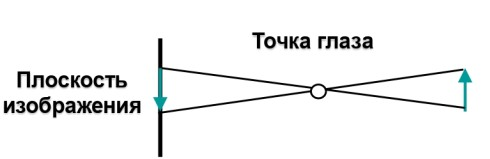
\includegraphics[width=\textwidth]{l5/S022.jpg}
		\caption{Реальная камера}
	\end{subfigure}
	\begin{subfigure}[b]{0.45\textwidth}
		\centering
		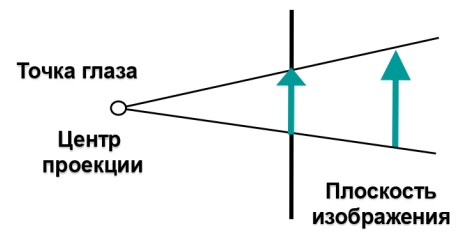
\includegraphics[width=\textwidth]{l5/S023.jpg}
		\caption{Подходящий эквивалент в КГ}
	\end{subfigure}
	\caption{Камера в графике}
\end{figure}
В реальном мире изображение формируется на задней поверхности камеры, в компьютерной графике - изображение формируется перед объективом камеры.

\subsubsection{Преобразования камеры}
Упростим, перемещая точку зрения камеры в центр, таким образом, чтобы смотреть в направлении отрицательной оси $Z$.

\subsection{Перспективное проектирование}
\screenshot{width=9cm}{l5/S024.jpg}{Перспективная проекция}
\begin{itemize}
	\item Подобность реальному миру
	\item Характеризуется видимым в перспективе объектом
	\item Объекты кажутся большими, если они ближе к камере
	\item Что необходимо:
	\begin{itemize}
		\item Центр проектирования
		\item Плоскость проектирования
	\end{itemize}
	\item Проектирование: соединение объекта к центру проектирования
\end{itemize}
\textbf{Картинная плоскость} определяется некоторой точкой на плоскости, которую будем называть \textbf{опорной точкой} (ОТ) и
нормалью к картинной плоскости (НКП). 

\screenshot{width=9cm}{l5/S025.jpg}{Проекция}

КП может произвольным образом располагаться относительно проецируемых объектов, заданных в мировых координатах. Она может пересекать их, проходить впереди или  позади объектов.

Для того, чтобы задать окно, нам необходима система координат, которую назовём системой координат $UV$. Началом ее служит ОТ.

Направление оси $V$ на КП определяет \textbf{вектор вертикали} (ВВ) - проекция ВВ на КП совпадает с осью $V$.

ОТ и два направления вектора НКП и ВВ определяются d правосторонней мировой системе координат. Имея на КП систему $UV$, можем задать минимальное и максимальное значения $U$ и $V$, определяющие окно — поле вывода.

В случае центральной проекции ВО определяется также центром проекции. Этот параметр задается в мировых координатах относительно ОТ.

\subsubsection{Область представления}
\screenshot{width=9cm}{l5/S026.jpg}{Область представления}
Определяет, сколько из мира взято в картину. Чем больше область представления, тем меньше размер объекта проектирования

\subsubsection{Передняя и задняя плоскости отсечения}
\screenshot{width=9cm}{l5/S027.jpg}{Плоскости отсечения}
\begin{itemize}
	\item Выводятся только объекты между передней (near) и задней (far) плоскостями отсечения. 
	\item Передняя плоскости отсечения + задняя плоскости отсечения +	объем видимости = пространство видимости
	
\end{itemize}

\FloatBarrier
\subsection{Графический конвейер}
В большинстве подсистем трехмерной графики применяется графический конвейер. \textbf{Конвейер} - это логическая группа вычислений, выполняемых последовательно, которые дают на выходе синтезируемую сцену. Наличием переходов между этапами конвейера обеспечивается возможность выбора между программной и аппаратной реализацией очередного этапа

Такой подход к настройке конвейера позволяет приложениям трехмерной графики получать преимущества аппаратной реализации, когда таковая доступна. Таким образом, реализация конвейера может чисто программной, полностью аппаратной или смешанной (программно-аппаратной)

\subsubsection{Состав графического конвейера}
На входе:
\begin{itemize}
	\item \textbf{Геометрическая модель}: Описание всех объектов, поверхностей и геометрии источников света и преобразований
	\item \textbf{Световая модель}: Описания вычислительные свойств объектов и источников света
	\item \textbf{Точка наблюдения (или камера)}: Позиция наблюдателя и угол обзора
\end{itemize}

Собственно, конвейер:
\begin{enumerate}
	\item Модельные преобразование
	\item Освещение (Закраска, Shading)
	\item Видовое преобразование (Перспектива)
	\item Отсечение (Clipping)
	\item Проецирование в экранное пространство
	\item Растеризация (Rasterization)
	\item Видимость (Вывод)
\end{enumerate}

Растровый вывод - пиксельная решетка, куда выводится изображение. Может быть в формате цвет/интенсивность.

\subsubsection{Модельные преобразования}
\begin{itemize}
	\item Трехмерные модели определены в их собственной системе координат (объектное пространство - object space)
	\item Моделирование преобразовывает модели в пределах общей координационной структуры (мировое пространство - world space)
\end{itemize}
\screenshot{width=\textwidth}{l5/S028.jpg}{Пространство объекта и мировое пространство}

\subsubsection{Освещение (закраска)}
Вершины освещены (закрашены, затенены) согласно свойствам материала, свойствам поверхностей (нормали) и источникам света
\screenshot{width=9cm}{l5/S029.jpg}{Различные модели освещения}

\subsubsection{Видовое преобразования}
\subparagraph{Для чего нужно еще одно преобразование?}
Проективные преобразования описывают «стандартные» проекции, т.е. проецируют фиксированную часть пространства
\subparagraph{Что если мы хотим переместить наблюдателя?}
Варианты:
\begin{itemize}
	\item Изменить матрицу проекции, чтобы включить в нее информации о камере
	\item Применить дополнительное преобразование, «подгоняющее» объекты под стандартную камеру
\end{itemize}
Стандартная камера в OpenGL:
\begin{itemize}
	\item Наблюдатель в $(0, 0, 0)$
	\item Смотрит по направлению $(0, 0, -1)$
	\item Верх $(0, 1, 0)$
\end{itemize}

Мировое пространство преобразовывается в видовое.
Положение наблюдателя, преобразованное к центру и направлению, сориентировано вдоль некоторой оси (обычно 2)

\subsubsection{Отсечение (Clipping)}
\screenshot{width=9cm}{l5/S030.jpg}{Отсечение}
Преобразует в нормализованные координаты устройства. Части объекта вне объема представления удалены.

\subsubsection{Проецирование}
Объекты проецируются в пространство изображения (экранное пространство
\screenshot{width=9cm}{l5/S031.jpg}{Проецирование}

\subsubsection{Растеризация}
Объекты растеризуются в пиксели.
\screenshot{width=12cm}{l5/S032.jpg}{Растеризация}

\subsubsection{Видимость / Вывод}
Каждый пиксел помнит самый близкий объект (буфер глубины).

Почти каждый шаг в графическом конвейере вызывает изменение системы координат. Преобразования являются центральными к пониманию трехмерной компьютерной графики.

\subsubsection{Координатные системы в конвейере}
\begin{tabular}{|l|l|l|}
	\hline
	\textbf{Этап конвейера} & \textbf{Координатные системы} \\
	\hline
	Модельные преобразование & Object Space \\
	\hline
	Освещение (Закраска, Shading) & World Space \\
	\hline
	Видовое преобразование (Перспектива) & Eye Space \\
	\hline
	Отсечение (Clipping) & Clip Space (NDC)\\
	\hline
	Проецирование в экранное пространство & Screen Space\\
	\hline
	Растеризация (Rasterization) &\\
	\hline
	Видимость (Вывод) & \\
	\hline
\end{tabular}

\subsubsection{Координатные системы}
\begin{itemize}
	\item Объектное пространство — объектная система координат.\\
	Локальное для каждого объекта
	\item Мировое пространство - мировая система координат\\
	Общее для всех объектов
	\item Видовое пространство / Камера — видовая система координат\\
	Выводится из области видимости
	\item Пространство отсечения / нормализованное пространство устройства(NDC) - НСК\\
	$[-1,-1,-1]$ > $[1,1,1]$
	\item Экранное пространство — экранные координаты\\
	индексируется в соответствии с атрибутами hardware
\end{itemize}

\subsubsection{Концептуальная модель процесса 3D-вывода}
\screenshot{width=12cm}{l5/S033.jpg}{3D-вывод}

\FloatBarrier
\subsubsection{Картинная плоскость}
\screenshot{width=12cm}{l5/S034.jpg}{Картинная плоскость}
\begin{itemize}
	\item \textbf{Картинная плоскость} \\Характеризуется:
	\begin{itemize}
		\item Опорной точкой
		\item Нормалью к картинной плоскости
		\item Расстоянием до картинной плоскости (КП)
	\end{itemize}
	\item \textbf{Опорная точка}\\
	Определяет картинную плоскость. Берется в МК, обычно принадлежит объекту или находится внутри него (ТПВ — точка привязки вида (VRP view reference point).
	\item \textbf{Расстояние до КП} - расстояние от опорной точки в направлении вектора нормали картинной плоскости
	\item \textbf{Нормаль к картинной плоскости} - задает ориентацию картинной плоскости. Для однозначного задания положения камеры недостаточно знать ориентацию картинной плоскости, так как остается еще одна степень свободы камеры — поворот вокруг нормали к картинной плоскости. Задание вектора вертикали вид ВВКП зафиксирует однозначно ориентацию камеры.
\end{itemize}

\subsection{Простейшая перспективная проекция}
Спроектируем все точки вдоль оси $z$ к плоскости $z=d$, точка наблюдения в НК:
\screenshot{width=6cm}{l5/S035.jpg}{Простейшая проекция}
$$
\dfrac{x_p}{d} = \dfrac{x}{z + d}; \ \dfrac{y_p}{d} = \dfrac{y}{z+d}
$$
$$
x_p = \dfrac{d \cdot x}{z + d} = \dfrac{x}{\frac{z}{d} + 1}
$$
$$
y_p = \dfrac{d \cdot y}{z + d} = \dfrac{y}{\frac{z}{d} + 1}
$$
Представление обобщённой спроектированной точки: $
P_p=\begin{bmatrix} X & Y & Z & W \end{bmatrix}^T
$. В таком случае то же самое в матричном виде:
$$
P_p = M_{per} \cdot P = \begin{bmatrix}
1 & 0 & 0 & 0\\
0 & 1 & 0 & 0\\
0 & 0 & 1 & 0\\
0 & 0 & \frac{1}{d} & 0
\end{bmatrix} 
\cdot \begin{bmatrix} x \\ y \\ z \\ 1 \end{bmatrix} 
= \begin{bmatrix} X & Y & Z & W \end{bmatrix}^T = 
\begin{bmatrix} x & y & z & z/d \end{bmatrix}^T
$$
\subsection{Виды плоских геометрических проекций}
По расположению центра проекции относительно плоскости проекции различаются \textbf{центральная} и \textbf{параллельная} проекции.
\screenshot{width=9cm}{l5/S036.jpg}{Центральная и параллельная проекции}

Центральная проекция имеет центр проекции, а параллельная проекция не имеет центра проекции, т.е. считается, что этот центр располагается в бесконечности.

\screenshot{width=\textwidth}{l5/S037.jpg}{Виды проекций}

Параллельные проекции делятся на два типа в зависимости от соотношения между направлением проецирования и нормалью к проекционной плоскости:
\begin{itemize}
	\item \textbf{ортографические} - направления совпадают, т. е. направление проецирования является нормалью к проекционной плоскости;
	\item \textbf{косоугольные} - направление проецирования и нормаль к проекционной плоскости не совпадают.
\end{itemize}

\subsubsection{Мультивидовая ортографическая}
\screenshot{width=9cm}{l5/S038.jpg}{Мультивидовая ортографическая проекция}
Используются для:
\begin{itemize}
	\item Технических рисунков машин, машинных частей
	\item рабочие архитектурные рисунки
\end{itemize}

Доводы "за":
\begin{itemize}
	\item точное возможное измерение
	\item все представления в том же самом масштабе
\end{itemize}

Доводы "против":
\begin{itemize}
	\item не обеспечивает "реалистическое" представление или смысл трехмерной формы
\end{itemize}

$$
M_{orth} = \begin{bmatrix}
1 & 0 & 0 & 0\\
0 & 1 & 0 & 0\\
0 & 0 & 0 & 0\\
0 & 0 & 0 & 1
\end{bmatrix} 
$$

\subsubsection{Аксонометрические проекции}
Тот же самый метод как мультивидовое орфографическое проектирование, кроме того, что плоскости проектирования не параллельны любой из координатных плоскостей; параллельные линии одинаково видятся в перспективе
\begin{itemize}
	\item \textbf{Изометрическая}: углы между всеми тремя основными осями равны (120°). Одинаковые отношения масштаба применяются вдоль каждой оси
	\item \textbf{Диметрическая}: углы между двумя из основных осей равны; отношения масштаба применяются вдоль двух осей
	\item \textbf{Триметрическая}: углы, различные между тремя основными осями; три отношения масштаба
\end{itemize}
Триметрическая: углы, различные между тремя основными осями; три отношения масштаба
\screenshot{width=9cm}{l5/S039.jpg}{Аксонометрическая проекция}
Наиболее общей формой является изометрическая проекция. Расстояние по всем трем главным осям укорачивается с одним и тем же коэффициентом, поэтому возможно с одним и тем же масштаб коэф. по всем трем осям. Для ее образования нужно одинаковое число раз сократить все три оси.
$$
\begin{bmatrix}
\cos{\phi} & \sin{\phi} \cdot \sin{\theta} & -\sin{\phi} \cdot \cos{\theta} & 0 \\
0 & \cos{\theta} & \sin{\theta} & 0\\
\sin{\phi} & -\cos{\phi} \cdot \sin{\theta} & \cos{\phi} \cdot \cos{\theta} & 0\\
0 & 0 & 0 & 1
\end{bmatrix}
$$

\subsubsection{Косоугольные проекции}
\screenshot{width=9cm}{l5/S040.jpg}{Косоугольные проекции}
Косоугольные проекции Кавалье и Кабине не сохраняют ортогональности системы координат. Данные проекции нечасто используются в инженерной практике.

\textbf{Кавалье} (Военная проекция): две оси кажутся перпендикулярными и не сокращены; третья ось наклонена по отношению к горизонтали (на угол 45°) и не сокращена

\textbf{Кабине}: угол между проекторами и плоскостью проекции $arctan(2)=63.4^\circ$. Взаимно перпендикулярные плоскости 	проецируются с коэффициентом 50%

\subsubsection{Совмещенное представление видов параллельных проекций}
\begin{itemize}
	\item Многовидовая ортография
	\begin{itemize}
		\item VPN паралельна всем осям
		\item DOP паралельна VPN
		\item Видна вся грань
	\end{itemize}
	\item Аксонометрическая проекция
	\begin{itemize}
		\item VPN не паралельна осям кооординат
		\item DOP параллельна VPN
		\item Изменяется размер. Размер — функция угла между нормалью грани и DOP
	\end{itemize} 
	\item Косоугольная проекция
	\begin{itemize}
		\item VPN паралельна основной координатной оси
		\item DOP не паралельна VPN
		\item Изменение граней за исключением параллельной КП
	\end{itemize}
\end{itemize}

\subsubsection{Центральная проекция}
\screenshot{width=\textwidth}{l5/S041.jpg}{Пирамида видимости}
\screenshot{width=\textwidth}{l5/S042.jpg}{Виды перспектив в центральной проекции}
\end{document}
